%%%%%%%%%%%%%%%%%%%%%%%%%%%%%%%%%%%%%%%%%%%%%%%%%%%%%%%%%%%%%%%
%%%  dts notes
%%%%%%%%%%%%%%%%%%%%%%%%%%%%%%%%%%%%%%%%%%%%%%%%%%%%%%%%%%%%%%%

\documentclass[onecolumn,fleqn]{revtex4}

% fonts
\usepackage{latexsym}
\usepackage{amsmath} 
\usepackage{amssymb} 
\usepackage{bm}
\usepackage{wasysym}

\usepackage{graphicx}


% extra by jarondl
\usepackage{array}
\usepackage{float}%unfloats
%\usepackage{multicol}
\usepackage[caption=false]{subfig} %subcaption is not compat with revtex
\usepackage[pdftitle={PTA},bookmarks]{hyperref}


%%%%%%%%%%%%%%%%%%%%%%%%%%%%%%%%%%%%%%%%%%%%%%%%%%%%%%%%%%%%%%%%

% NEW 
\newcommand{\abs}[1]{\left|#1\right|}
\newcommand{\varphiJ}{\bm{\varphi}}
\newcommand{\thetaJ}{\bm{\theta}}
%\renewcommand{\includegraphics}[2][0]{FIGURE}
\newcommand{\rmrk}[1]{\textcolor{red}{#1}}
\newcommand{\Eq}[1]{\textcolor{blue}{Eq.\!\!~(\ref{#1})}} 
\newcommand{\Fig}[1]{\textcolor{blue}{Fig.}\!\!~\ref{#1}}

% math symbols I
\newcommand{\sinc}{\mbox{sinc}}
\newcommand{\const}{\mbox{const}}
\newcommand{\trc}{\mbox{trace}}
\newcommand{\intt}{\int\!\!\!\!\int }
\newcommand{\ointt}{\int\!\!\!\!\int\!\!\!\!\!\circ\ }
\newcommand{\ar}{\mathsf r}
\newcommand{\im}{\mbox{Im}}
\newcommand{\re}{\mbox{Re}}

% math symbols II
\newcommand{\eexp}{\mbox{e}^}
\newcommand{\bra}{\left\langle}
\newcommand{\ket}{\right\rangle}

% Mass symbol
\newcommand{\mass}{\mathsf{m}} 
\newcommand{\rdisc}{\epsilon} 

% more math commands
\newcommand{\tbox}[1]{\mbox{\tiny #1}}
\newcommand{\bmsf}[1]{\bm{\mathsf{#1}}} 
\newcommand{\amatrix}[1]{\begin{matrix} #1 \end{matrix}} 
\newcommand{\pd}[2]{\frac{\partial #1}{\partial #2}}

% equations
\newcommand{\mylabel}[1]{\label{#1}} 
\newcommand{\beq}{\begin{eqnarray}}
\newcommand{\eeq}{\end{eqnarray}} 
\newcommand{\be}[1]{\begin{eqnarray}\ifthenelse{#1=-1}{\nonumber}{\ifthenelse{#1=0}{}{\mylabel{e#1}}}}
\newcommand{\ee}{\end{eqnarray}} 

% arrangement
\newcommand{\hide}[1]{}
\newcommand{\drawline}{\begin{picture}(500,1)\line(1,0){500}\end{picture}}
\newcommand{\bitem}{$\bullet$ \ \ \ }
\newcommand{\Cn}[1]{\begin{center} #1 \end{center}}
\newcommand{\mpg}[2][1.0\hsize]{\begin{minipage}[b]{#1}{#2}\end{minipage}}
\newcommand{\mpgt}[2][1.0\hsize]{\begin{minipage}[t]{#1}{#2}\end{minipage}}

%%%%%%%%%%%%%%%%%%%%%%%%%%%%%%%%%%%%%%%%%%%%%%%%%%%%%%%%%%%%%%%%%%%%%%%%%%%
% Sections
\newcommand{\sect}[1]
{
\addtocounter{section}{1} 
\setcounter{subsection}{0}
\ \\ 
\pdfbookmark[2]{\thesection. \ #1}{sect.\thesection}
{\Large\bf $=\!=\!=\!=\!=\!=\;$ [\thesection] \ #1}  
\nopagebreak
}

% subections
\newcommand{\subsect}[1]
{
\addtocounter{subsection}{1} 
\ \\ 
\pdfbookmark[2]{\ \ \ \ \thesection.\thesubsection. \ #1}{subsect.\thesection.\thesubsection}
{\bf $=\!=\!=\!=\!=\!=\;$ [\thesection.\thesubsection] \ #1}  
\nopagebreak
}
%%%%%%%%%%%%%%%%%%%%%%%%%%%%%%%%%%%%%%%%%%%%%%%%%%%%%%%%%%%%%%%%%%%%%%%%
%%%%%%%%%%%%%%%%%%%%%%%%%%%%%%%%%%%%%%%%%%%%%%%%%%%%%%%%%%%%%

\graphicspath{{figures/}}
\begin{document}

\title{PTA}

\author{YdL}

\maketitle

%%%%%%%%%%%%%%%%%%%%%%%%%%%%%%%%%%%%%%%%%%%%%%%%%%%%%%%%%%%%%%%%%%%%%%%%
%%%%%%%%%%%%%%%%%%%%%%%%%%%%%%%%%%%%%%%%%%%%%%%%%%%%%%%%%%%%%%%%%%%%%%%%


%%%%%%%%%%%%%%%%%%%%%%%%%%%%%%%%%%%%%%%%%%%%%%%%%%%%%%%%%%%
\sect{Model}

A periodic banded logbox model. The band profile is flat ($\Theta(b)$).
The off diagonal elements are log-box:
%
\begin{align}
w_{nm} &= w_0 \eexp{-\epsilon} \\
\epsilon &\in \textrm{uniform  } [0,2\sigma]
\end{align}
%
The diagonal elements are set so that each row's sum will be zero.
%
\begin{align}
w_{nn} = -\sum_{m\ne n} w_{nm}  
\end{align}
%
%%%%%%%%%%%%%%%%%%%%%%%%%%%%%%%%%%%%%%%%%%%%%%%%%%%%%
\sect{PN plots}

We have produced several plots of PN vs $\lambda$. For low-sparsity, there is an 
agreement with the two "windows" observation. (For very low sparsity there are even hints
of three windows). It seems that the effect of sparsity is to shorten the more extended window,
up to a point where very few modes are extended (remember that the special $\lambda=0$ is always fully extended).


\begin{figure}[H]
  \subfloat[Low sparsity]{
    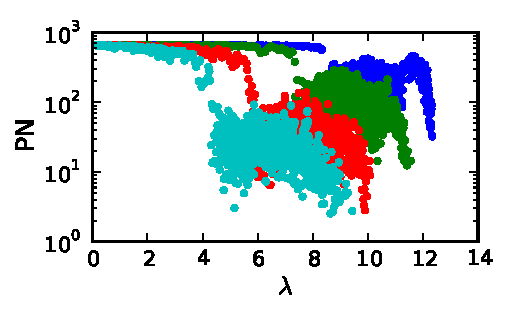
\includegraphics{pta_low_s_nopin}
    
  }
  \subfloat[Sparse]{
    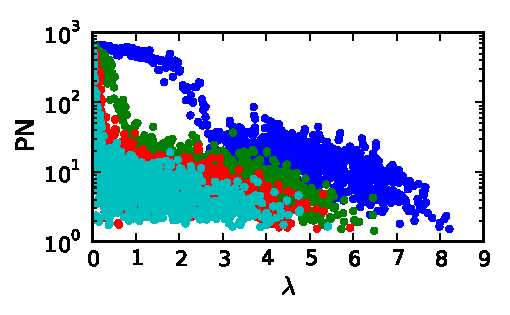
\includegraphics{pta_higher_s_nopin}
    
  }
  \\
  \subfloat[Very sparse]{
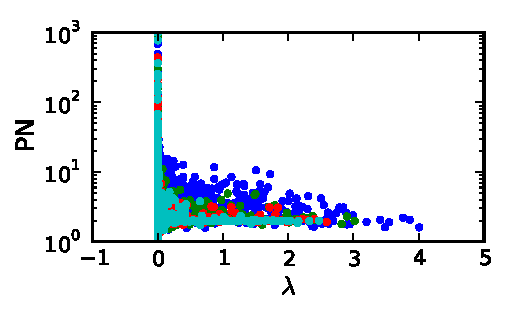
\includegraphics{pta_highest_s_nopin}
    
  }
\subfloat[Very sparse - logscale]{
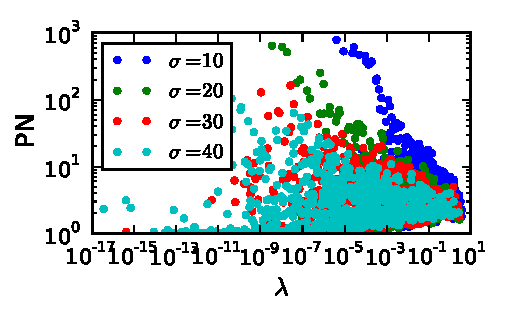
\includegraphics{pta_highest_s_log_nopin}
    
  }
  \caption{{\bf PN} as a function of $\lambda$ for sparse systems.
  For all the plots $N=1000$ and $b=5$}
\end{figure}



%%%%%%%%%%%%%%%%%%%%%%%%%%%%%%%%%%%%%%%%%%%%%%%%%%%%%%%%%%%%%%%%%%%%
\sect{The effects of pinning}

By pinning we mean adding some elements to the diagonal,
that represent a spring attaching a ball to a fixed origin.


We used a uniform distribution on the range $[-0.3,0]$,
in order to discern the effect.


It seems that the only difference is some localization in
the low-eigenvalues. The lowest modes are replaced with less 
extended modes with higher eigenvalues. Note that the $\lambda=0$ mode no longer
exist. To highlight the low eigenvalues,
we have used log-scale for the $\lambda$ axis.

\begin{figure}[H]
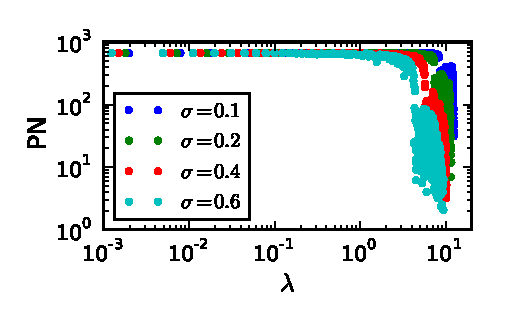
\includegraphics{pta_low_s_log_nopin}
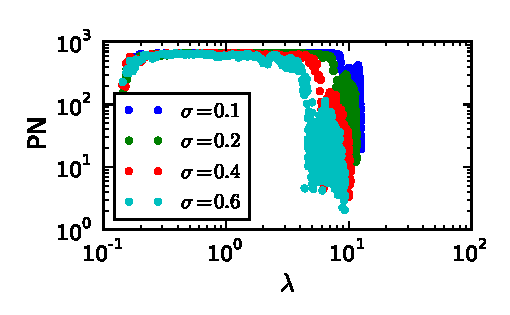
\includegraphics{pta_low_s_log_pin}
\caption{On the left, without pinning, and on the right with pinning}
\end{figure}


 
%%%%%%%%%%%%%%%%%%%%%%%%%%%%%%%%%%%%%%%%%%%%%%%%%%%%%%%%%%%%%%%%%%%
\sect{Thouless conductance}

Extended modes are more sensitive to boundary conditions. To measure
the effect quantitivly, we've used Thouless' method of adding
a phase to the boundary condition, and measuring the change in the eigenvalues.

We define $\lambda_0$ as the eigenvalue with regular periodic boundary conditions,
and $\lambda_\phi$ as the eigenvalue after applying a phase of $\phi$ to the boundary conditions.
Then $g$ is defined as
%
\begin{align}
  g = \frac{|\lambda_\phi - \lambda_0 |}{\phi^2}\ \times \ \frac{1}{\Delta}
\end{align}
%
Where $\Delta\ =\ \lambda_{n+1}-\lambda_n$ is the level spacing. 
In practice, we have averaged over five 
neighboring spacings to avoid artifacts.


The resulting $g(\lambda)$ is strikingly similar to the $PN(\lambda)$ results,
but the change is much stronger (note the logarithmic $y$-scale).  


\begin{figure}[H]
  \subfloat[Low sparsity]{
    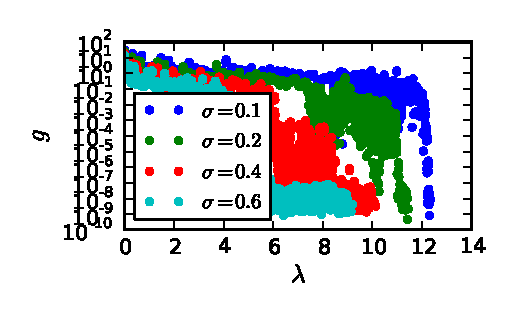
\includegraphics{pta_thouless_low_s}
    
  }
  \subfloat[Sparse]{
    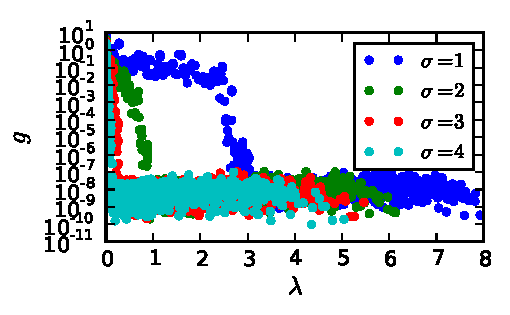
\includegraphics{pta_thouless_higher_s}
    
  }
  \\
  \subfloat[Very sparse]{
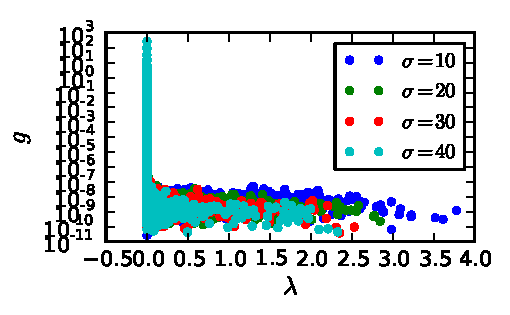
\includegraphics{pta_thouless_highest_s}
    
  }
\subfloat[Very sparse - logscale]{
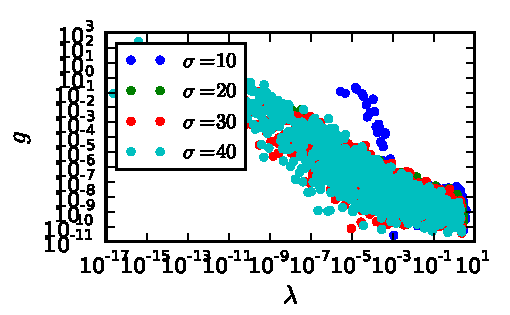
\includegraphics{pta_thouless_highest_s_log}
    
  }
  \caption{$g$ as a function of $\lambda$ for sparse systems.
  For all the plots $N=1000$ and $b=5$}
\end{figure}

%%%%%%%%%%%%%%%%%%%%%%%%%%%%%%%%%%%%%%%%%%%%%%%%%%%%%%%%%%%%%%%%%%%%%%%%%
\sect{Diagonal Disorder}


In the RP we have claimed that the conservation of the matrix
causes the very wide modes on the lower edge of the spectrum.
To see this point, we ran numerics with $N=1000$ $b=5$ and $\sigma=0.1$.

 Also notice the arc-like feature on the right,
it was there previously, but it is more pronounced for $\sigma=0.1$.  
The plateau is for $PN=\frac{2}{3}N$, as is expected for a cosine wave. 


Conservation means that the sum of each row is zero, so that the diagonal is minus the
sum of all other terms. The first way to break conservation is by adding
random elements to this diagonal.
\begin{align}
\gamma_n = -\sum_m w_{nm} + w_0\eexp{-\varepsilon}
\end{align}
 In the plot legends we mark this by the removal of $C$.
 
 
Another way is by neglecting to do the sum altogether,
keeping only:
\begin{align}
\gamma_n = + w_0\eexp{-\varepsilon}
\end{align}
In the plot legends we mark this by adding $D$.



In \autoref{fig:pta_sym1} we see the resulting $PN$ and $g$. We see
that the lowest eigenmodes behave differently. To examine this effect,
we have shifted the $x$ axis by the minimal $\lambda$, and applied log-scale.
For the conserving matrix, the $PN$ is constant in the low eigenvalues. The
uncoserving matrix has a small decline, and the one without special diagonal 
has a larger decline. 




\begin{figure}[H]
  \subfloat[g]{
    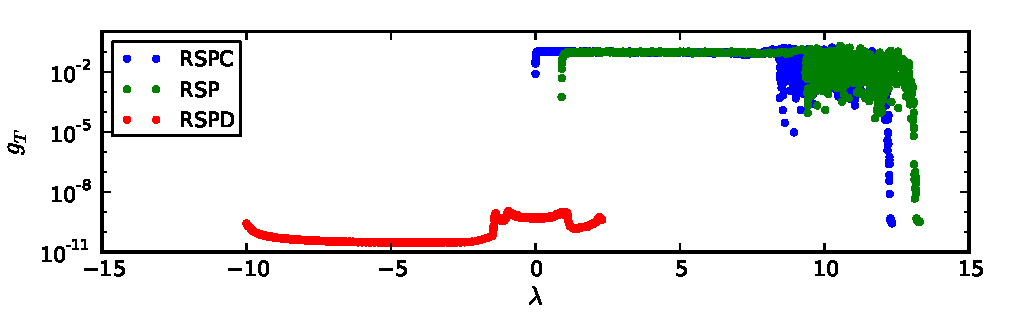
\includegraphics{pta_sym_neg_g}  
    
  }\\
  \subfloat[PN]{
    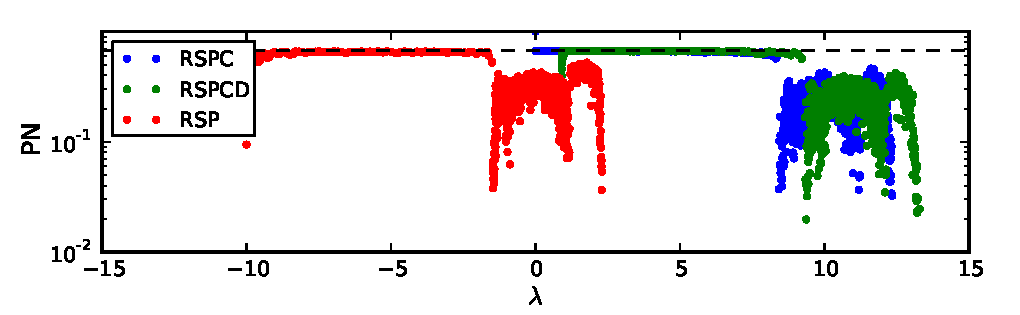
\includegraphics{pta_sym_neg_PN}
    
  }\\
  \subfloat[PN around zero]{
    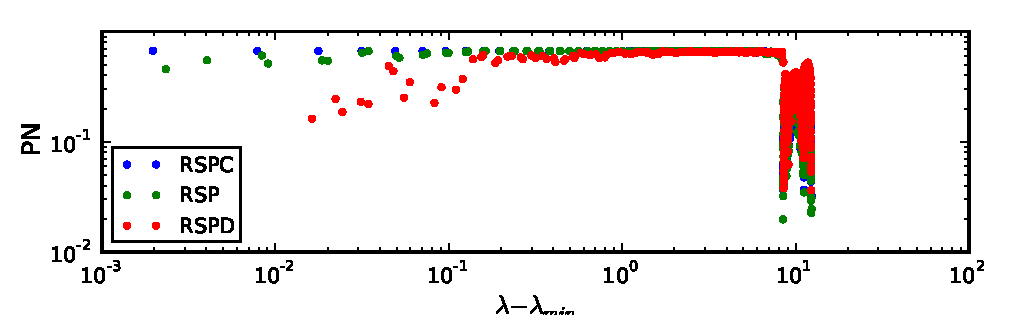
\includegraphics{pta_sym_neg_PN_zero}
    
  }
  \caption{$g$ and PN as a function of $\lambda$ for sparse systems.
  For all the plots $N=1000$, $b=5$ and $\sigma=0.1$. 
  The label codes are R-Real S-Symmetric P-[Positive Elements] C-Conservative D-[no-special diagonal] .
  The dashed line is on $y=2/3$, the expected PN for a cosine wave.}
  \label{fig:pta_sym1}
\end{figure}

%%%%%%%%%%%%%%%%%%%%%%%%%%%%%%%%%%%%%%%%%%%%%%%%%%%%%%%%%%%%%
\sect{non positive elements}

Here we check the effects of positivity on the $PN$ structure. We multiply
the matrix elements by a random sign $[\pm 1]$, keeping it symmetric.
The change from before is striking, as the plateau vanishes completely.

We examine the conservation aspects here as well, with the same
too measures of diagonal disorder. We see that when we do not treat the diagonal
specially, there are no wide modes at all. For the conserving and disorder matrices,
there are some wide modes. In the conserving case they are around the center, with a $\lambda=0, PN=N$ mode.
For the non-conserving mode this behavior shifts to the right. To further
analyze this area, we have shifted the $x$-axis, and plotted only the points to the 
right of the peak, to allow log-scale. The other half is symmetric. 
\begin{figure}[H]
  \subfloat[g]{
    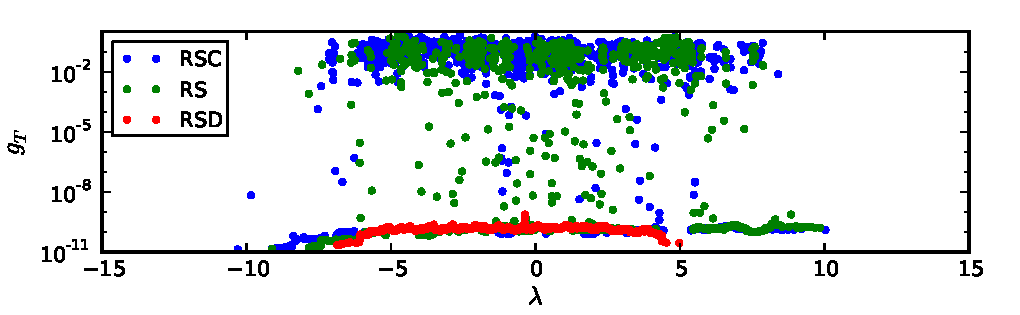
\includegraphics{pta_sym_neg_g2}  
    
  }\\
  \subfloat[PN]{
    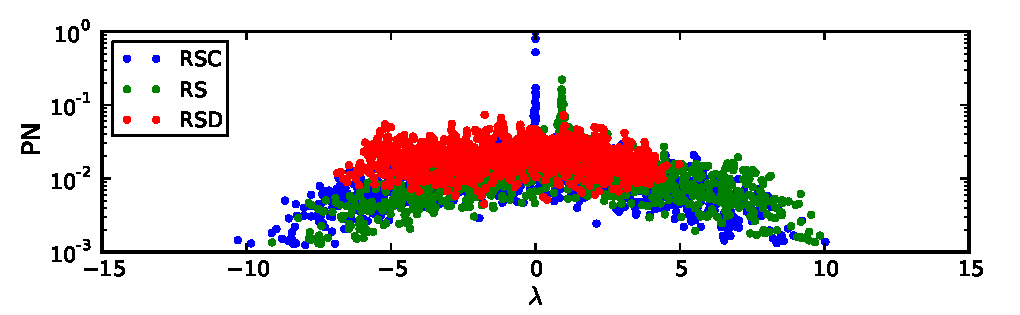
\includegraphics{pta_sym_neg_PN2}
    
  }\\
  \subfloat[PN around center]{
    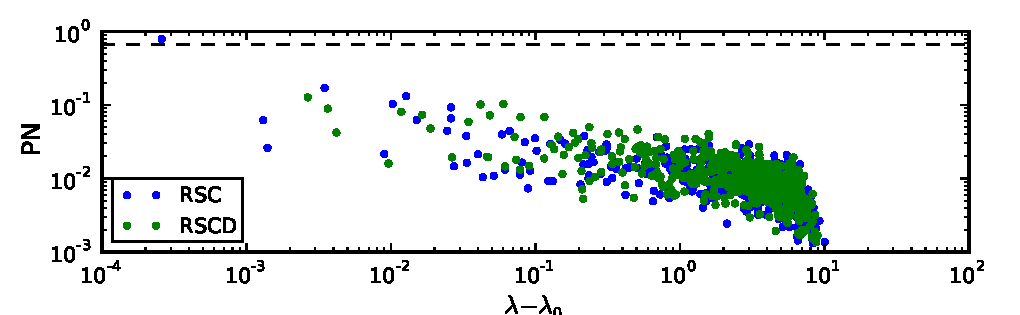
\includegraphics{pta_sym_neg_PN_center}
    
  }
  \caption{$g$ and PN as a function of $\lambda$ for sparse systems.
  For all the plots $N=1000$, $b=5$ and $\sigma=0.1$. 
  The label codes are R-Real S-Symmetric P-[Positive Elements] C-Conservative D-[no-special diagonal] . Note
  that the last plot has only half of the points}
  \label{fig:pta_sym2}
\end{figure}


%%%%%%%%%%%%%%%%%%%%%%%%%%%%%%%%%%%%%%%%%%%%%%%%%%%%%%%%%%%%%%%%%%%%%
\sect{Relating mean free path to DOS}

We mark the Density-Of-States by $\varrho_\lambda$.
According to FGR, the transition rate,
or the inverse of mean-free-time is
\begin{align}
\frac{1}{t_\ell} = \varrho_\lambda w_{nm}
\end{align}
the mean-free-path is:
\begin{align}
\ell = v_\lambda t_\ell = \frac{v_\lambda}{\varrho_\lambda w_{nm}}
\end{align}
For $v_\lambda$ we could probably take the Fermi velocity.


Next, we need to connect the mean-free-path with the localization length 
in 1-3d. Basically, in $1d$ they are the same,
with 
\begin{align}
\xi\sim \ell
\end{align}
For banded $1d$ we expect
\begin{align}
\xi \sim b^2 \ell
\end{align}

In $2d$ there is an exponential dependence on $g$ (?),
\begin{align}
\xi\sim \eexp{g} \ell
\end{align}
While in $3d$ we have the $\beta$-function:
\begin{align}
\beta(g) = \frac{\partial g}{\partial \log(L)}
\end{align}
If $\beta(g)>0$, then the derivative is positive, and the RG flow
goes to the right, and vice versa. For $3d$ there is
a critical $g_c=1$, where to the right of it $\beta(g)>0$, and 
to the left $\beta(g)<0$. This means that if $g_0>1$, the localization
length diverges, and if $g_0<1$ the localization length goes to $0$.


An interesting question is the relation between the wavelength and
the localization length. If the localization length is smaller then
the wavelength it has no meaning.
%%%%%%%%%%%%%%%%%%%%%%%%%%%%%%%%%%%%%%%%%%%%%%%%%%%%%%%%%%%%%%%%%%%%%%%
\sect{Band structure}

We can find the DOS at the ends of the bands,
and their inverse should be the localization length.

Perhaps, because of a special matrix feature or some symmetry,
we have extended states with lower energy, similar in idea
to cooper pairs in super-conductors.


%%%%%%%%%%%%%%%%%%%%%%%%%%%%%%%%%%%%%%%%%%%%%%%%%%%%%%%%%%%%%%%%%%%%%%%%
\sect{Anderson Localization Length - numerical}

According to Tal Weiss' summary, the localization length
for the $1d$ case with $w_{ij}=1$, and $\gamma_i = [-s,s]$, is:
\begin{align}
 l = 2 \ \frac{4 - E^2}{\sigma} 
 \end{align}
where $\sigma$ is the variance of the $\gamma$ distribution. 
In our case $\sigma = \frac{s^2}{3}$, leading us to:
\begin{align}\label{eq:anderson_l}
 l = 6 \ \frac{4-E^2}{s^2} 
 \end{align}
we check this numerically in three simple ($b=1$) cases:
\begin{enumerate}
    \item{For the Anderson model with $w_{ij}=1$, and $\gamma_i = [-s,s]$ in \autoref{fig:anderson}.}
    \item{For the "Anderson-rate" model with$\gamma_i=0$ and $w_{ij}= 1 + \left[-\frac{s}{2}, \frac{s}{2} \right]$
            in \autoref{fig:anderson_rate}}
    \item{For the "Anderson-rate" conserving model with the same rates but $\gamma_i = -\sum_j w_{ij}$
            in \autoref{fig:anderson_rate_conserv}}
\end{enumerate}

To understand the band structure, it helps to first think of the analytical 
solution of the ordered state.
Without disorder, the eigenvectors and eigenvalues are:
\begin{align}
k\ \  &=\ \  \frac{\pi m}{N} \ \ \ \ \ m=1..N \\
\vec{V}_k\ \  &=\ \  \cos(k\cdot x)\\
\lambda_k\ \  &=\ \  2\cos(k) \ \ \ \ \ \ (+2 \textrm{  for conserving matrix)}
\end{align}  
All of these eigenvectors have $PN\ =\ (2/3)N$.
This is marked in the plots by a horizontal dashed line. 
The eigenvalues are confined between $-2$ and $2$  (add $2$ for conserving matrix).
The density of states for the ordered model is:
%
\begin{align}
\textrm{DOS} = \frac{1}{v} = \left(\frac{d\lambda_k}{dk}\right)^{-1} = -\frac{1}{2\sin(k)} = -\frac{1}{\sqrt{4-\lambda^2}}
\end{align}
Note that this has two diverging points, at $E=\pm 2$.


The localization length for weak disorder is 
\begin{align}
\ell = 2\cdot\frac{v^2}{\sigma}= 2\cdot\frac{4-\lambda^2}{\sigma}
\end{align}



\begin{figure}[H]
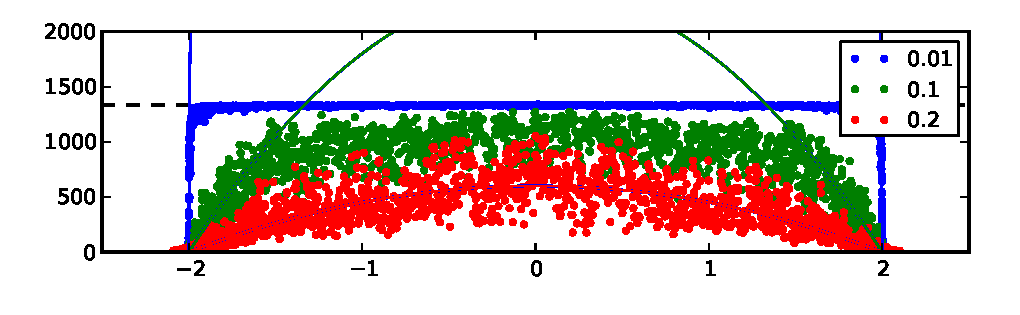
\includegraphics{pta_anderson_b1}\\
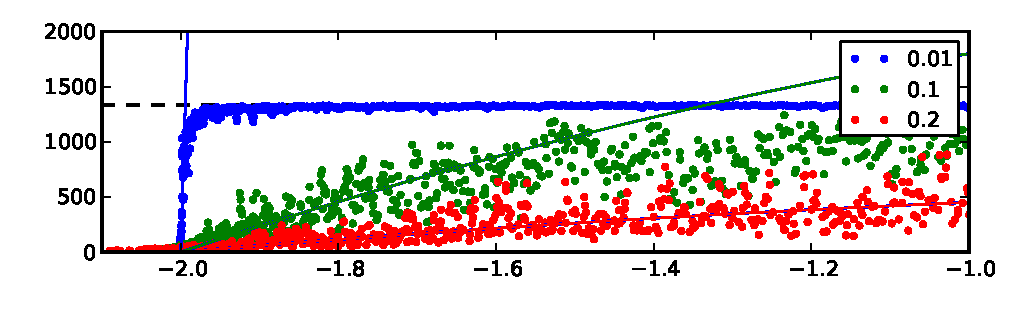
\includegraphics{pta_anderson_b1_zoom}
\caption{PN vs. eigenvalues for the plain Anderson model ($w_{ij}=1$, $\gamma_i = [-s,s]$), 2000 sites. 
The lines are according to \autoref{eq:anderson_l}
}\label{fig:anderson}
\end{figure}

\begin{figure}[H]
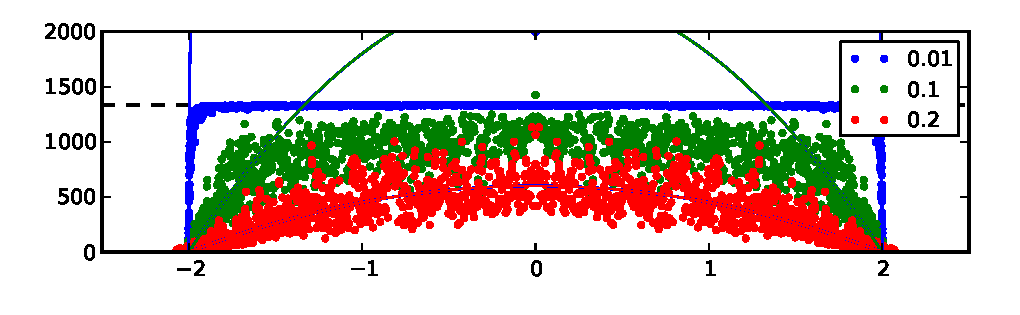
\includegraphics{pta_anderson_rates_b1}\\
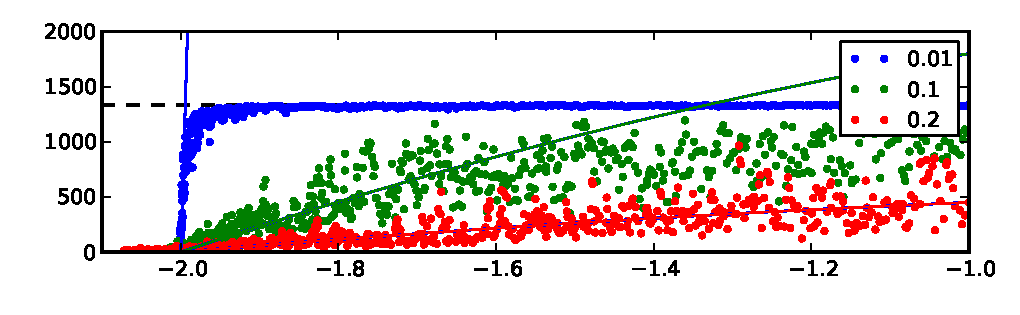
\includegraphics{pta_anderson_rates_b1_zoom}
\caption{PN vs. eigenvalues for the "Anderson-Rate" model ($\gamma_i = 0$, $w_{ij} = 1 + \left[-\frac{s}{2}, \frac{s}{2}\right]$), 2000 sites. 
The lines are according to \autoref{eq:anderson_l}
}\label{fig:anderson_rate}
\end{figure}

\begin{figure}[H]
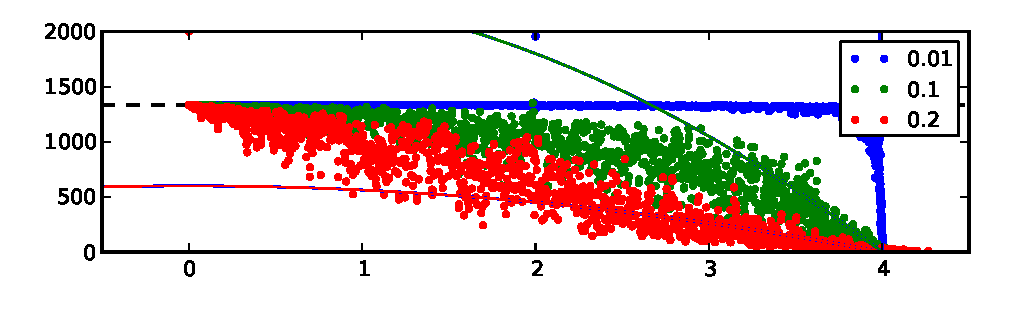
\includegraphics{pta_anderson_rates_conserv_b1}\\
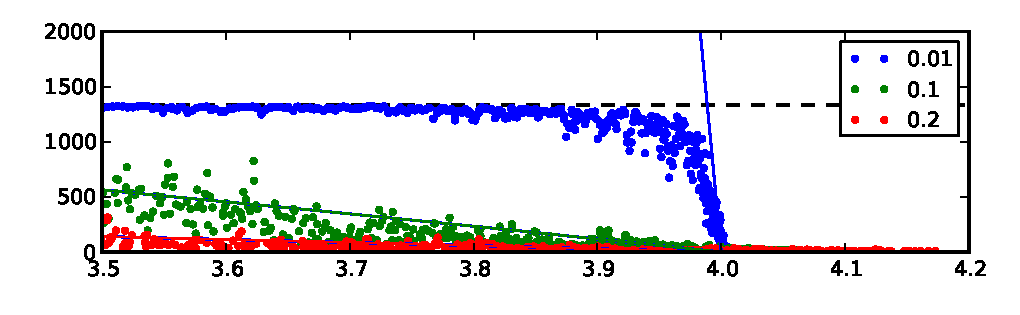
\includegraphics{pta_anderson_rates_conserv_b1_zoom}
\caption{PN vs. eigenvalues for the "Anderson-Rate" conserving model ( $w_{ij} = 1 + \left[-\frac{s}{2}, \frac{s}{2}\right]$), 2000 sites. 
The lines, which don't fit exactly, are a variation of \autoref{eq:anderson_l}, with $E\rightarrow \frac{1}{2}\ E$.
}\label{fig:anderson_rate_conserv}
\end{figure}

%%%%%%%%%%%%%%%%%%%%%%%%%%%%%%%%%%%%%%%%%%%%%%%%%%%%%%%%%%%%%%%%%%%%%%%%
\sect{Banded matrices}

Before we move forward with disordered  banded matrices, let
us start with ordered ones.
The eigenvectors don't change (Bloch's theorem is still valid), but the eigenvalues do:
\begin{align}
k\ \  &=\ \  \frac{\pi m}{N} \ \ \ \ \ m=1..N \\
\vec{V}_k\ \  &=\ \  \cos(k\cdot x)\\
\lambda_k\ \  &=\ \  \sum_{n=1..b} 2\cos(n\cdot k) \ \ \ \ \ \ (+2b \textrm{  for conserving matrix)}
\end{align}  
The velocity is now:
\begin{align}
v \ \ &=\ \ \frac{d\lambda_k}{dk} \ \ =\ \ -\sum_{n=1..b} 2\cdot n\cdot \sin(n\cdot k)
\end{align}
There are $b+1$ points where $v=0$. 
The lowest eigenvalue is when $k=0$, $\lambda = -2b$.
The highest is tougher to calculate.

Let us analyze the one around $k=0$. 
In second order in $k$ , we have:
\begin{align}
\lambda &= \sum_{n=1..b} 2(\cos(n\cdot k)) \approx \sum_{n=1..b} 2-(n\cdot k)^2 \\
&=2b-\frac{1}{6} b(b+1)(2b+1) k^2\\
v\ \ &\approx -\sum_{n=1..b} 2\cdot n\cdot n \cdot k = \left(-\sum_{n=1..b} 2\cdot n\cdot n \right) k \\
&=-\frac{2}{6} b(b+1)(2b+1) k \\
v^2 &\approx \frac{2}{3}b(b+1)(2b+1)  (2b-\lambda)
\end{align}

\begin{figure}[H]
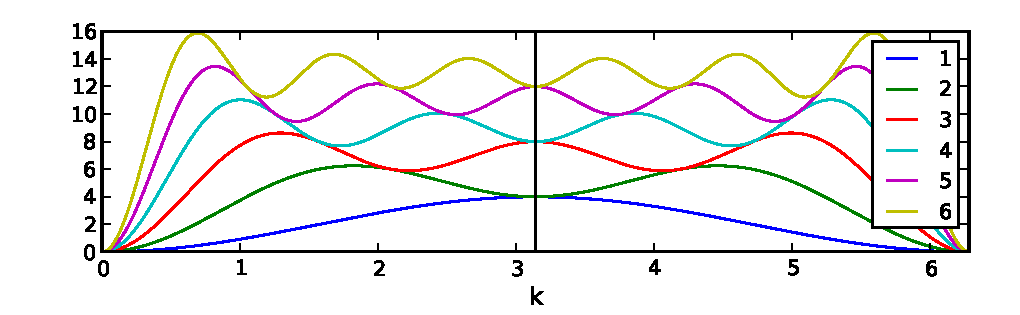
\includegraphics{pta_theor_banded_ev}
\caption{Theoretical eigenvalues for banded ordered matrices. Since our 
models are periodic, only the left half of this picture is relevant.
We can see that there are $b+1$ points where $v=0$ or the DOS diverges.
}\label{fig:theor_banded_ev}
\end{figure}


\begin{figure}[H]
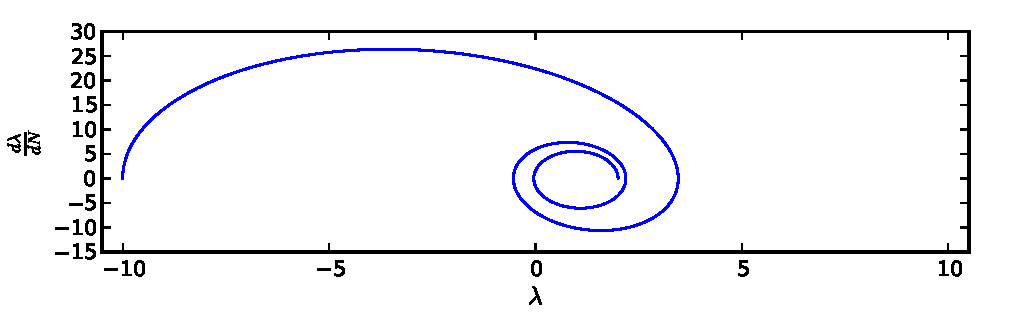
\includegraphics{pta_theor_banded_dos}
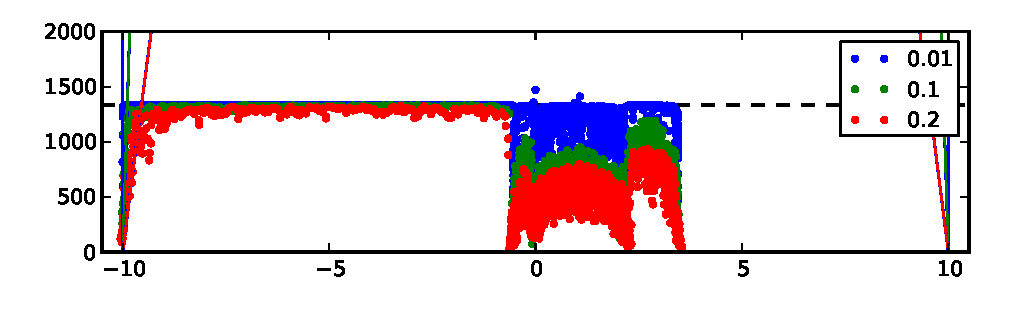
\includegraphics{pta_anderson_rates_b5}\\
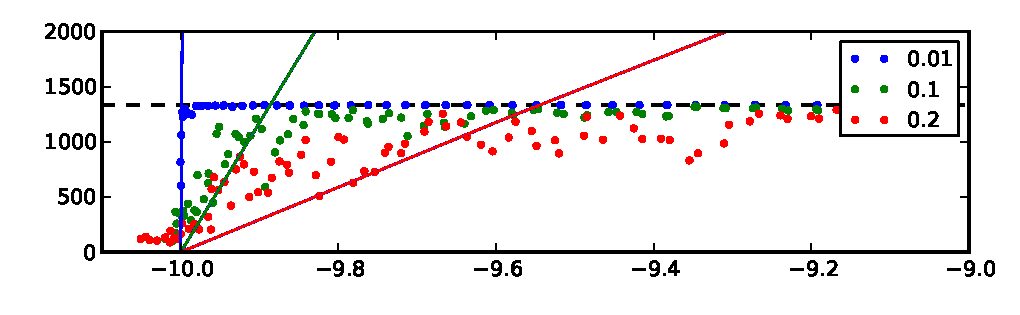
\includegraphics{pta_anderson_rates_b5_zoom}
\caption{PN vs. eigenvalues for the "Anderson-Rate" model $b=5$.
 The top plot is of velocity $v=\frac{d\lambda}{dk}$ vs eigenvalues $\lambda$. The DOS is the inverse of this.
In the other two plots, the lines are simply $\frac{2 v^2}{\sigma}$. Notice that
there is more then one $k$ for each $\lambda$. 
}\label{fig:anderson_rate_b5}
\end{figure}

\begin{figure}[H]
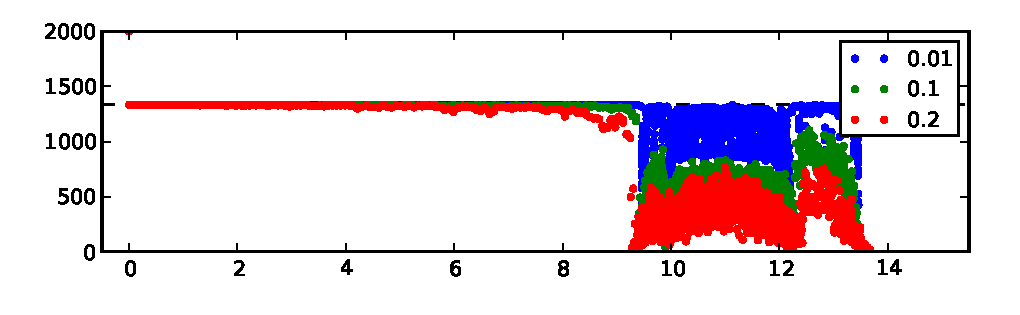
\includegraphics{pta_anderson_rates_conserv_b5}
\caption{PN vs. eigenvalues for the "Anderson-Rate" conserving model $b=5$.
The near zero localization is gone.
}\label{fig:anderson_rate_conserv_b5}
\end{figure}
\end{document}
